Afin d'assurer le bon fonctionnement de tous les cas différents, incluant la propagation directe, la réflexion simple, la double réflexion et la transmission, les valeurs obtenues ont été reprises et comparées aux résultats de la simulation. Les rayons ont également été dessinés pour s'assurer que la correspondance avec les résultats attendus soit exacte et que tout soit correct. \footnote{Tous les graphes de ce chapitre sont en grande taille en Annexe A.}


\section{Equations générales pour les différents cas}
La propagation directe peut être modélisée par l'équation suivante:
\begin{equation}
\underline{E_n} = \Gamma_1 \Gamma_2 \Gamma_3 \ldots T_1 T_2 T_3 \ldots \sqrt{60 G_{TX}(\theta_{TX_n},\phi_{TX_n}) P_{TX}} \frac{e^{-j\beta d_n}}{d_n}
\end{equation}
où $\Gamma_i$ et $T_i$ représentent respectivement les coefficients de réflexion et de transmission.

\subsubsection{Puissance reçue}
La puissance reçue par le récepteur est donnée par l'équation suivante:
\begin{equation}
P_{RX} = \frac{1}{8Ra} \left|\sum_{n=1}^{N} \vec{h_e^{RX}}\left(\frac{\pi}{2}, \phi_n\right) \underline{E_n}(\vec{r})\right|^2
\end{equation}
$\theta = \frac{\pi}{2}$ est utilisé pour les calculs, car une adaptation parfaite et une polarisation perpendiculaire sont supposées.

\subsubsection{Impédance du mur et constante de propagation }
L'impédance du mur et la constante de propagation sont calculées à l'aide des formules suivantes, en considérant les propriétés électromagnétiques des matériaux:
\begin{align}
Z_m &= \sqrt{\frac{\mu_0}{\epsilon - j\sigma/\omega}} \approx (171.57 + j6.65) \, \Omega, \\
\gamma_m &= \alpha_m + j\beta_m = 1.55 + j39.90.
\end{align}
Ensuite les différents coefficients et angles dépendent du type de réflexions avec un obstacle et vont être comparés ci dessous.

\section{Visualisations et Comparaisons manuscrites et du simulateur}
\subsubsection{Visualisations}

Tout d'abord voici les tracés de rayons réalisés par le simulateur. Ceux-ci sont similaires à ceux de l'exercice du syllabus dont les tracés ne seront pas repris ici.
\begin{figure}[H]
\centering
\begin{subfigure}[b]{0.42\textwidth}
    \centering
    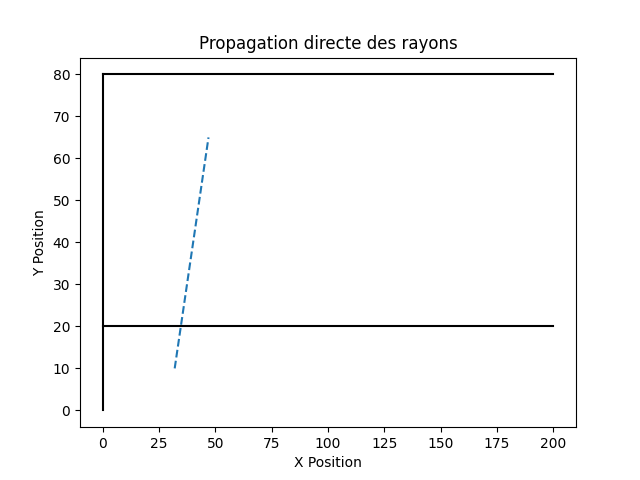
\includegraphics[width=\textwidth]{Pictures/propa_dir.png}
    \caption{Propagation directe \ref{fig:propd}}
    \label{fig:direct1}
\end{subfigure}
\hfill
\begin{subfigure}[b]{0.5\textwidth}
    \centering
    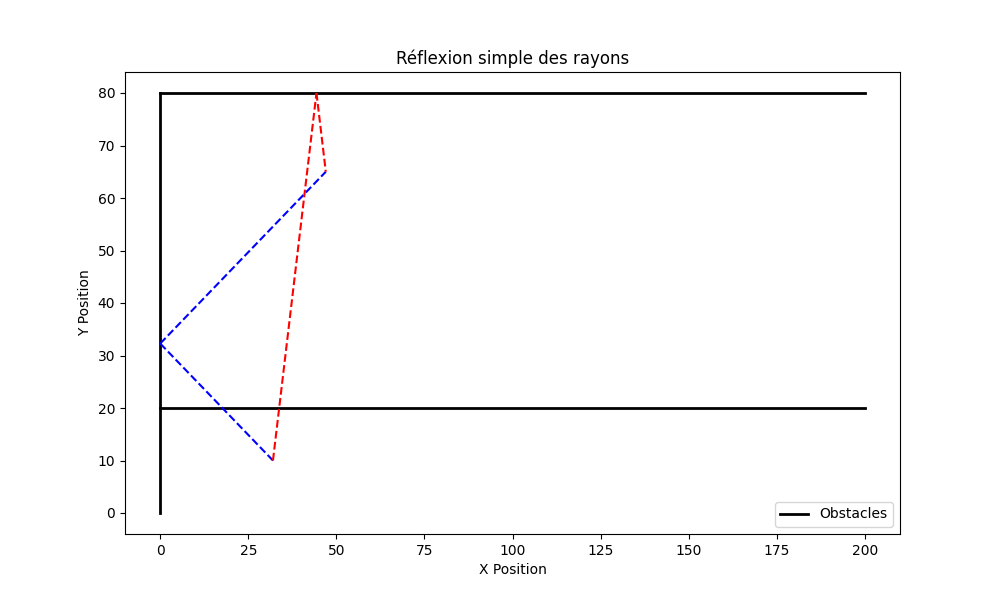
\includegraphics[width=\textwidth]{Pictures/simple_reflex.png}
    \caption{Réflexion simple \ref{refs}}
    \label{fig:simple_reflection}
\end{subfigure}

\begin{subfigure}[b]{0.45\textwidth}
    \centering
    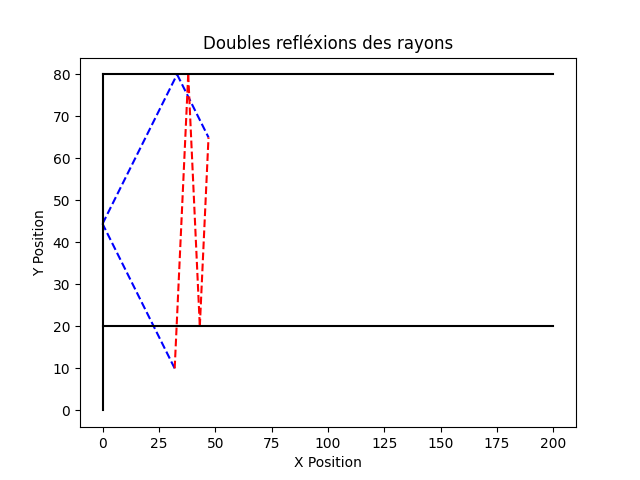
\includegraphics[width=\textwidth]{Pictures/double_reflex.png}
    \caption{Double réflexions \ref{refd}}
    \label{fig:double_reflection}
\end{subfigure}
\caption{Comparaison des différents types de propagation.}
\label{fig:ray_tracing}
\end{figure}

\subsubsection{Comparaison des Résultats}
Ci-dessous, le tableau comparant les valeurs obtenues manuellement avec celles de la simulation pour la propagation directe \ref{fig:direct1}.
\begin{table}[htbp]
\centering
\caption{Comparaison des résultats manuels et de simulation pour la propagation directe}
\label{tab:comparaison}
\begin{tabular}{@{}lcc@{}}
\toprule
\textbf{Paramètre} & \textbf{Valeur Manuelle} & \textbf{Valeur de Simulation} \\ \midrule
Champs Electrique (V/m) & $0.0037-0.0016j$ & $-0.0039994+3.8172944\times 10^{-5}j$ \\
Puissance reçue (W) &  $3.33 \times 10^{-10}$& $3.308468 \times 10^{-10}$ \\
Coefficient de transmission & $0.69+0.23j$ & $0.689195 + 0.237003j$ \\
Distance additionnelle parcourue (m) & $0.151$ & $0.151094$ \\
Angle d'incidence (degrés) & $15.2551$ & $15.255119$ \\
Angle de transmission (degrés) & $6.8796$ & $6.897650$ \\
Gamma perpendiculaire & $-0.3862+0.0165j$ & $-0.385931 + 0.016510j$ \\
$\gamma_m$ & $1.55+39.90j$ & $1.547482 + 39.872766j$ \\
Impédance du matériau $(\Omega)$ &$171.57+6.65j$& $171.683875 + 6.663138j$ \\
\bottomrule
\end{tabular}
\end{table} \\
La comparaison peut également être faite avec le cas à une réflexion pour le cas A (cas en bleu sur le graphe de la refléxion simple \ref{fig:simple_reflection}).
\begin{table}[htbp]
\centering
\caption{Comparaison des résultats manuels et de simulation pour la réflexion simple cas A}
\label{tab:comparaison_reflection}
\begin{tabular}{@{}lcc@{}}
\toprule
\textbf{Paramètre} & \textbf{Valeur Manuelle} & \textbf{Valeur de Simulation} \\ \midrule
Point d'impact ($P_r$) & $(0.0; 32.28)$ & $(0.0, 32.278481)$ \\
Angle d'incidence (degrés) & $34.8199$ & $34.84573$ \\
Angle de transmission (degrés) & $15.129$ & $15.1171208$ \\
Gamma perpendiculaire &$-0.4416+0.0156j$&$-0.441361+0.0156203j$\\
Coefficient de réflexion & $-0.334+0.225j$ & $-0.335708 + 0.225861j$ \\
Point d'impact ($P_t$) & $(17.64; 20)$ & $(17.636363;20)$ \\
Angle d'incidence (degré) & $55.1758$ & $55.1542665$ \\
Coefficient de transmission 1 (Émetteur $\rightarrow P_r$) & $0.539+0.023j$ & $0.537694 + 0.024983j$ \\
Distance additionnelle 1 (m) & $0.162$ & $0.161779$ \\
Coefficient de transmission 2 ($P_r \rightarrow$ récepteur) & $1+0j$ & $1.000000 + 0.000000j$ \\
Distance additionnelle 2 (m) & $0$ & $0.000000$ \\
Champs Electrique (V/m) & $-5.41\times 10^{-4}-4.57\times 10^{-4}j$ & $0.000441355+0.00055429153j $\\
Puissance reçue (W) &  $10.4 \times 10^{-12}$& $1.03829831227 \times 10^{-11}$ \\
\bottomrule
\end{tabular}
\end{table}\\
Pour les cas B à une reflexion et deux réflexion les résultats obtenus sont également ci dessous.\\
\begin{table}[H]
\centering
\caption{Comparaison des résultats manuels et de simulation pour les réflexions simple et doubles cas B}
\label{tab:comparaison_reflection}
\begin{tabular}{@{}lcc@{}}
\toprule
\textbf{Paramètre} & \textbf{Valeur Manuelle} & \textbf{Valeur de Simulation} \\ \midrule
cas B, réflexion simple & &\\ 
Champs Electrique (V/m) & $-4.52\times 10^{-4}-5.06\times 10^{-4}j$ & $0.000672792+0.00010809859j $\\
Puissance reçue (W) &  $9.5 \times 10^{-12}$& $9.6033123939 \times 10^{-12}$ \\
cas B, réflexion double & &\\ 
Champs Electrique (V/m) & $-7.86\times 10^{-5}-5.19\times 10^{-6}j$ & $-2.3403616\times 10^{-5} -7.614057941\times 10^{-5}j $\\
Puissance reçue (W) &  $0.1 \times 10^{-12}$& $1.3122870783 \times 10^{-13}$ \\
\bottomrule
\end{tabular}
\end{table}\\

Il est important de noter que les champs électriques sont différent pour les différents cas mais cela est dû à la grande variation de phase car l'émetteur est à $868.3 MHz$.\\
Après comparaison avec l'exercice 4.1 du syllabus du cours, les résultats sont similaire. Le simulateur est donc vérifié.